\documentclass[a4paper]{article}

\usepackage[utf8]{inputenc}
\usepackage[T1]{fontenc}
\usepackage{textcomp}
\usepackage[dutch]{babel}
\usepackage{amsmath, amssymb}
\usepackage{code}
\usepackage{pythonhighlight}
\usepackage{hyperref}
\hypersetup{
    colorlinks=true,
    linkcolor=blue,
    filecolor=magenta,      
    urlcolor=cyan,
    pdftitle={Overleaf Example},
    pdfpagemode=FullScreen,
    }
% figure support
\usepackage{import}
\usepackage{xifthen}
\usepackage{float}
\usepackage{gokul_pkg}
\pdfminorversion=7
\usepackage{pdfpages}
\usepackage{transparent}
\usepackage{graphicx}
\pdfsuppresswarningpagegroup=1
\graphicspath{{./img/}}

\begin{document}
\section{Digital 3D Lidar- Oster robotics Nicholous}
\subsection{what they do}
\begin{itemize}
	\item Industrial
	\item smart infrastructure
	\item robotics
	\item Automative
	      \begin{figure}[htpb]
		      \centering
		      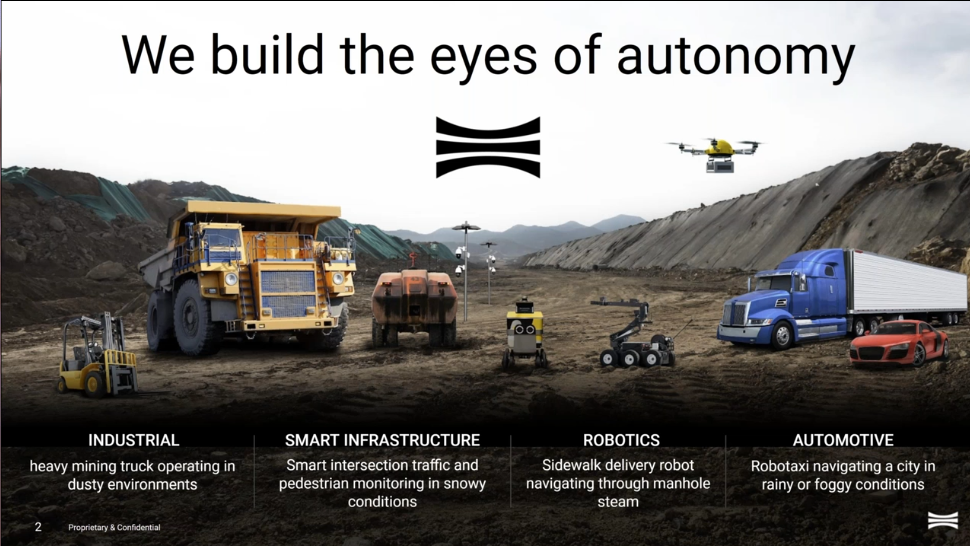
\includegraphics[width=0.8\textwidth]{whatOusterdo.png}
		      \caption{}
		      \label{fig:}
	      \end{figure}
\end{itemize}
\subsection{Why digital lidar}
\begin{itemize}
	\item  same as digital camera replaced analog cameras
	      \begin{figure}[H]
		      \centering
		      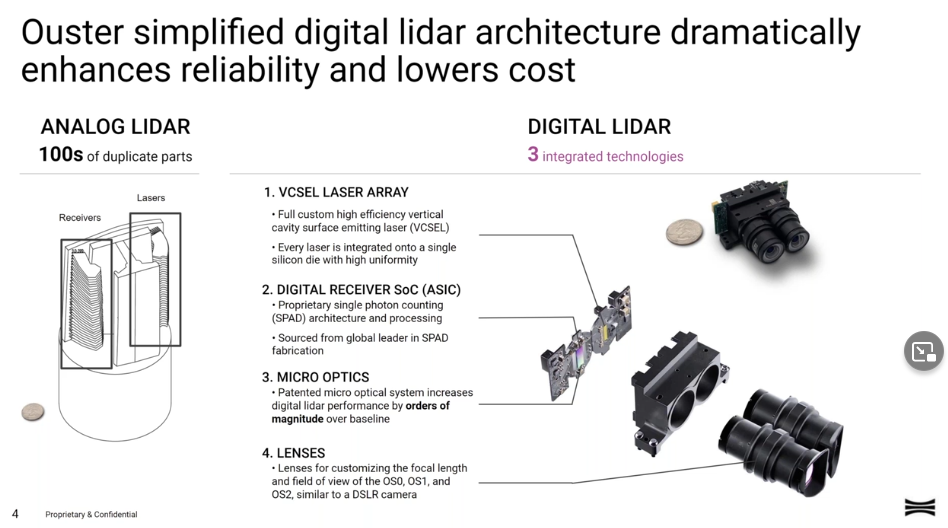
\includegraphics[width=0.8\textwidth]{whydigital.png}
		      \caption{}
		      \label{fig:}
	      \end{figure}
	\item 3 integerated technologies
	      \begin{itemize}
		      \item 1. VSCEL laser array(Vertical cavity surface emitting laser)
		      \item Every laser is in single die
	      \end{itemize}
\end{itemize}
\subsection{Their product}
\begin{figure}[htpb]
	\centering
	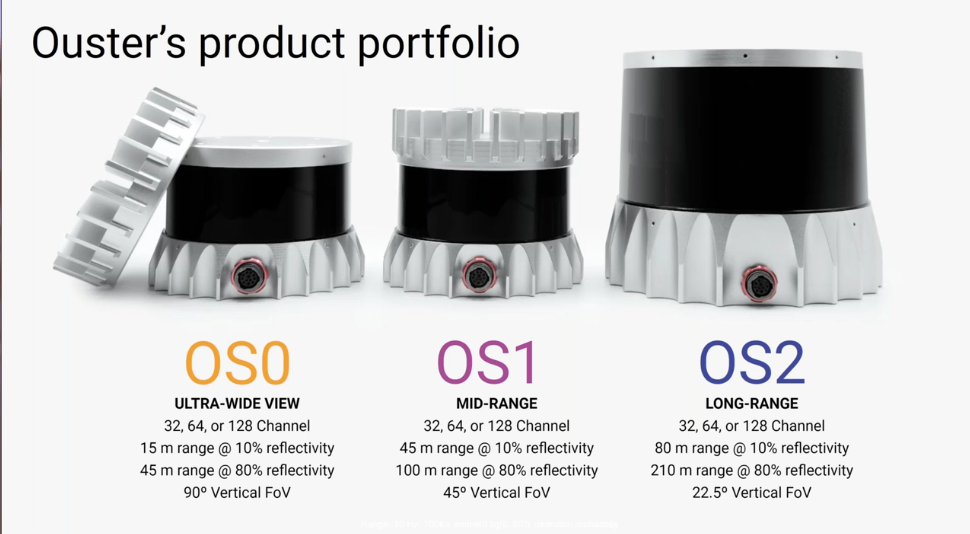
\includegraphics[width=0.8\textwidth]{ousterproducts.png}
	\caption{}
	\label{fig:}
\end{figure}
\subsection{Past warehouse automation}
\begin{itemize}
	\item Multi sensor suite
	      \begin{itemize}
		      \item Each task has its own sensor
		      \item 2d lidar and 3dTOf
		      \item Expensive and limiting technology,several points of failure
	      \end{itemize}
	\item Digital sensor can replace all senor to a single one
	      \begin{itemize}
		      \item reduce cost
		      \item improve localisation
		      \item high resolution(People can be seen clearly)
		      \item high field of view
	      \end{itemize}
\end{itemize}
\subsection{Improved localisation}
\begin{itemize}
	\item ULtrawide view
	\item maintain accurate postion in desolate area
	\item reduce lost robot downtime
	      \begin{figure}[htpb]
		      \centering
		      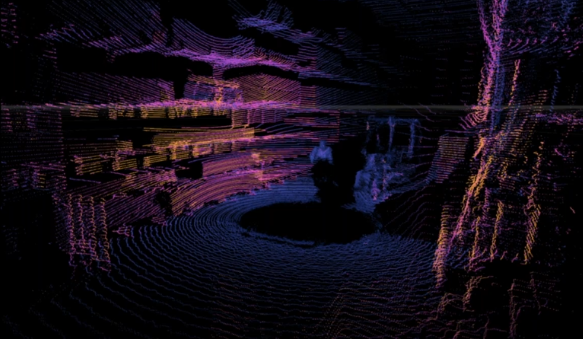
\includegraphics[width=0.8\textwidth]{digitalView.png}
		      \caption{}
		      \label{fig:}
	      \end{figure}
\end{itemize}
\subsection{Advanced perception}
\begin{itemize}
	\item Using high resolution provides robust perception
	\item Range,Signal,Near IR,calibirated reflectivity
	\item Next generation perception algorithms
\end{itemize}
\begin{itemize}
	\item Balyo warehouse,vecna robotics,has utilsed this sensors
	\item Can be used for object classification (partially)
	      \begin{figure}[H]
		      \centering
		      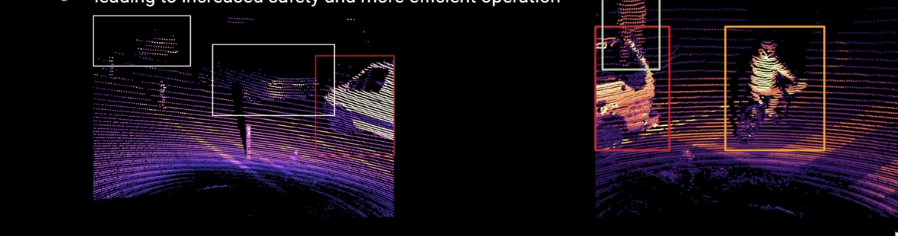
\includegraphics[width=0.8\textwidth]{objectClassification.png}
		      \caption{}
		      \label{fig:}
	      \end{figure}
\end{itemize}
\subsection{Final Notes}
\begin{itemize}

	\item ITS - fixed infrastructure for trafic management and accident detection same used inside warehouse for collision avoidance
	\item Will lidar be the next camera? - yes(accd to ouster)
	\item ros package is provide
	\item supplies to india(Indian listeners are here ;)  )
	\item ethernet communication
\end{itemize}
\newpage
\section{Thomas - sick sensors sensor fusion for navigation and perception}
\subsection{About}
\begin{itemize}
	\item Industrial lidars and sensors
	\item over the globe
	\item Creating sensor inteligence
	      \begin{figure}[htpb]
		      \centering
		      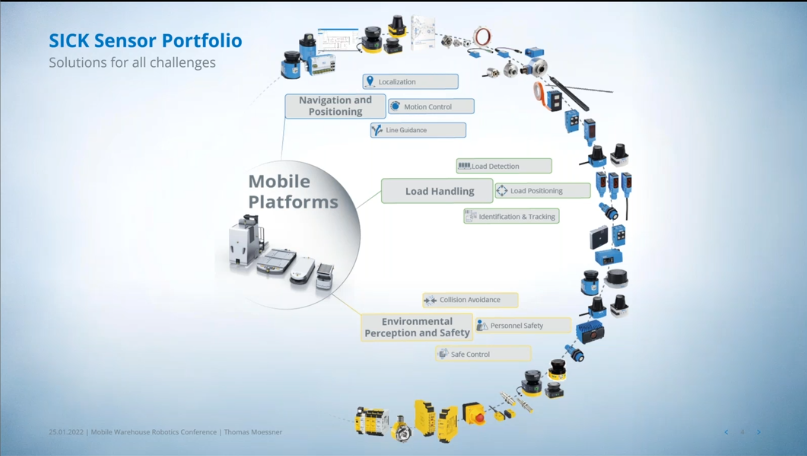
\includegraphics[width=0.8\textwidth]{sensotPortfolio.png}
		      \caption{}
		      \label{fig:}
	      \end{figure}
\end{itemize}
\subsection{Evolution of localisation}
\begin{itemize}
	\item long history of lidar sensor
	      \begin{figure}[htpb]
		      \centering
		      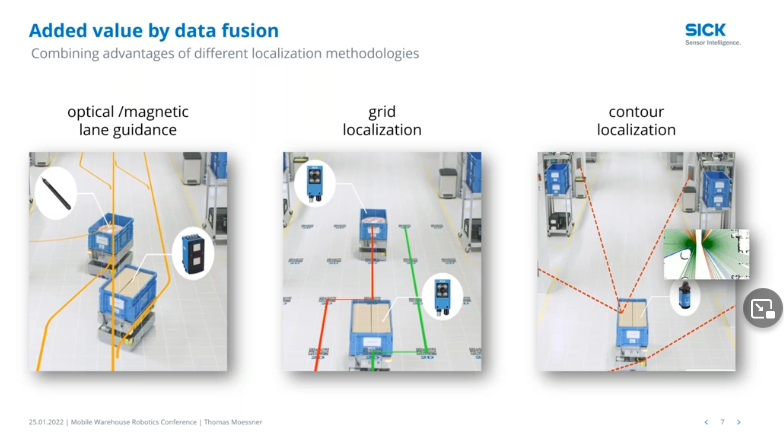
\includegraphics[width=0.8\textwidth]{datafusion.png}
		      \caption{}
		      \label{fig:}
	      \end{figure}
	\item fuse all three to get better performance
	\item contour -classic lidar localisation
\end{itemize}
\subsection{Vitual line localisation}
\url{https://www.youtube.com/watch?v=5IH-_PrQ7Io} \\
Use virtual lines for guiding the robots to move in path
\subsection{3d trolly position}
\begin{itemize}
	\item Typical load handiling postion
	\item fusing 3d lidar and 2d lidar
	\item capture with 3d lidar
	\item when trolley goes out of view for 3d lidar and 2d lidar can be used capture its postion
\end{itemize}
\section{Encoders for AGV - Nech Recelj RLS}
\subsection{About}
\begin{itemize}
	\item found in 1989
	\item rotary and linear encoders
	\item europe based country
	\item mission is to develop motion sensing components
\end{itemize}
\subsection{Types of guidance}
\begin{figure}[H]
	\centering
	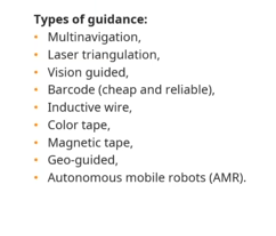
\includegraphics[width=0.8\textwidth]{guidance.png}
	\caption{}
	\label{fig:}
\end{figure}
AGV - uses fixed infrastructure \\
AMR - uses software to move freely in task space
\subsection{Types of steering in AGV}
\begin{itemize}
	\item Diff drive
	\item steer drive
	\item quad drive
\end{itemize}
\subsection{encoders}
\begin{itemize}
	\item \textbf{wheels} - incremental
	\item \textbf{steering} - absolute
	\item analog is best for certification
	      \begin{figure}[htpb]
		      \centering
		      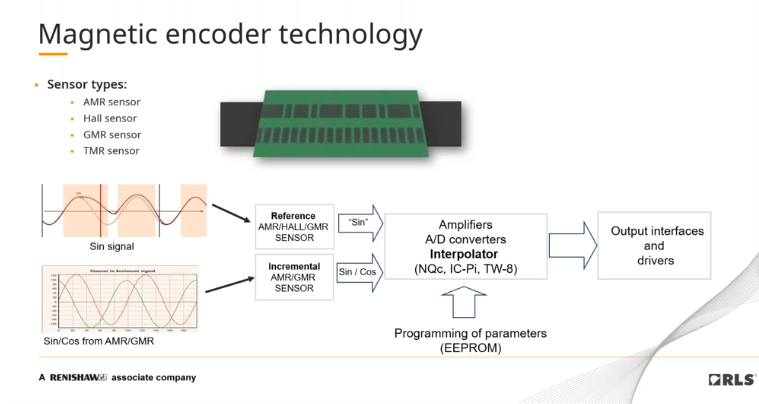
\includegraphics[width=0.8\textwidth]{magneticEncoder.png}
		      \caption{}
		      \label{fig:}
	      \end{figure}
	\item protocols
	      \begin{itemize}
		      \item SSI
		      \item BiSS C
		      \item CanOpen
	      \end{itemize}
\end{itemize}
\newpage
\section{Multi sensor fusion hub}
\subsection{About}
\begin{itemize}
	\item found in 2009
	\item fullstack hardware software and cloud analytics
	\item 33+ patents for motion sensing
	      \begin{figure}[H]
		      \centering
		      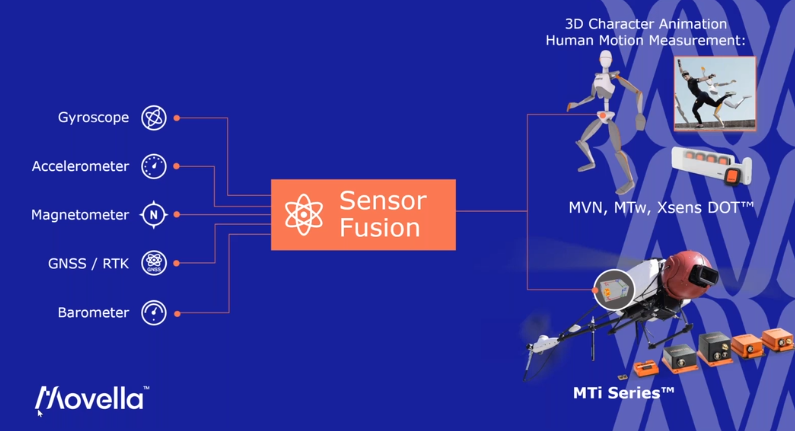
\includegraphics[width=0.8\textwidth]{sensorFusionMovella.png}
		      \caption{}
		      \label{fig:}
	      \end{figure}
\end{itemize}
\subsection{Multi sensor fusion hub}
\begin{itemize}
	\item challenges
	      \begin{itemize}
		      \item challenging structure
		      \item lighting conditions
		      \item Displacement of static objects
		      \item dynamic object controlled and uncontrolled
	      \end{itemize}
	\item sensor solutions
	      \begin{itemize}
		      \item Vision
		      \item Lidar
		      \item RFID
		      \item wifi
		      \item encoder
		      \item Bumpers
	      \end{itemize}
\end{itemize}
\subsection{IMUs}
\begin{itemize}
	\item Acceleromenter
	\item Gyro
	\item Magneto
	\item Application
	      \begin{itemize}
		      \item Heading control
		      \item Fall over protection
		      \item Load estimation
	      \end{itemize}
\end{itemize}
\subsubsection{Why IMUs}
\begin{itemize}
	\item precise dead reckoning
	\item better prediction
	\item reject outliers
	\item reacts to system failure
\end{itemize}
\newpage
\section{Our vision for adopting Edge AI in Autonomous Machines - eddie and terresa Nvidia}
\begin{itemize}
    \item Grace arm based cpu
    \item \textbf{Omniverse} - virtual world of photorealistic factory
\end{itemize}
\subsection{Robotics platform}
\subsubsection{challenges}
\begin{itemize}
    \item Expensive and time consuming
    \item sunstructured environment
    \item complex system with precise components
\end{itemize}
\subsubsection{Everything will become smarter}
\begin{itemize}
    \item anything built will have digital twin
    \item anything that moves will be autonomous
    \item anything autonomous will be simulated(mainly for taking datas)
\end{itemize}
\subsection{Isaac - nvidia robotics}
not a single sdk, combination of many things
\begin{figure}[H]
         \centering
         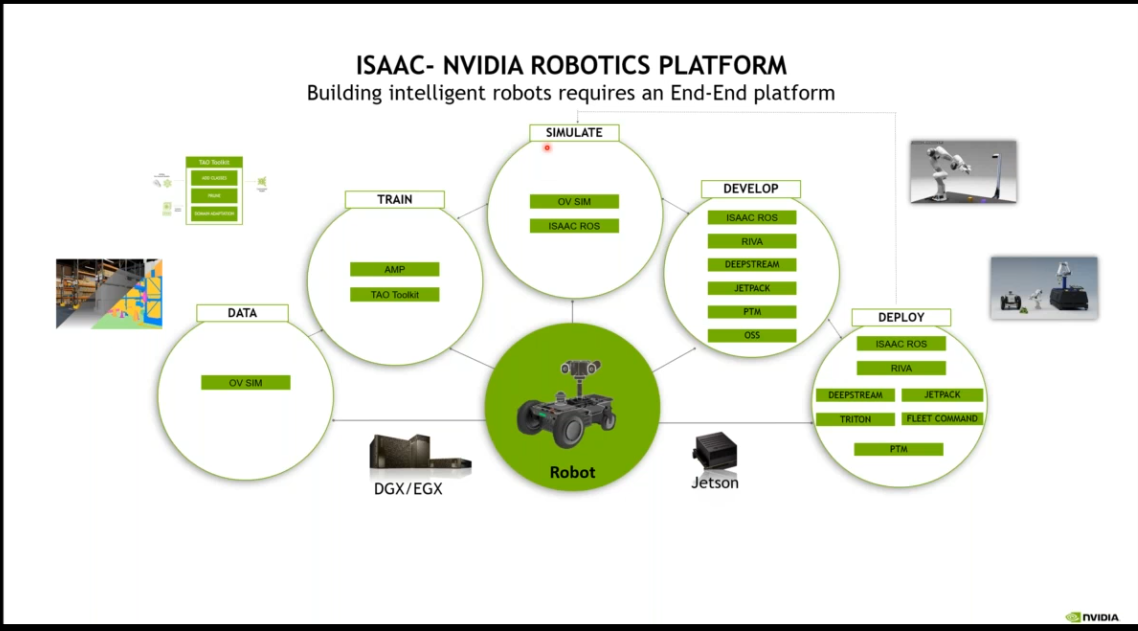
\includegraphics[width=0.8\textwidth]{issac.png}
         \caption{}
         \label{fig:}
     \end{figure}
\subsubsection{Development phases}
\begin{itemize}
    \item Data
    \item Train
    \item simulate
    \item develop
    \item deploy
\end{itemize}
\subsubsection{Isaac}
\begin{figure}[htpb]
          \centering
          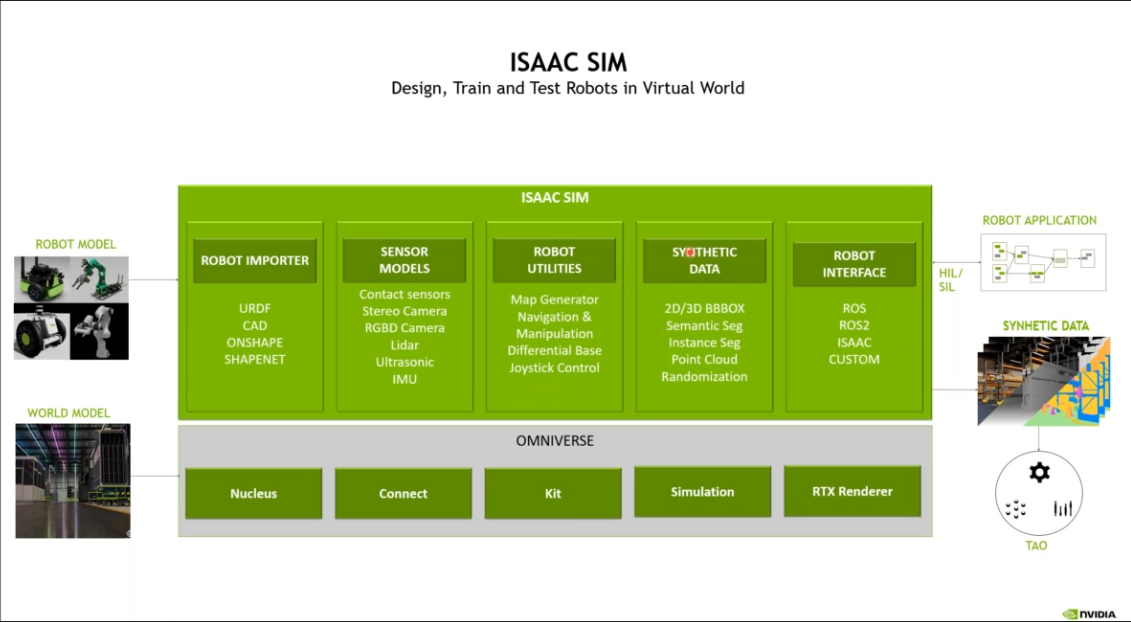
\includegraphics[width=0.8\textwidth]{isaacd.png}
          \caption{}
          \label{fig:}
      \end{figure}
      \begin{itemize}
          \item Synthetics sensors
          \item navigation simulation
          \item roboust dataset
          \item hardware accelerated for ROS
      \end{itemize}
\section{Future of ros}
\textbf{Rolling ridely} - daily update of ros \\
\textbf{humble hawksbil} - best for indutrial application 5 years of support \\
\textbf{OpenRMF} - framework for integerating multirobots and environments
\end{document}

